% =====================================================================
%  CAPÍTULO 5 — ARQUITETURA E DECISÕES DE PROJETO
% =====================================================================

\chapter[ARQUITETURA E DECISÕES DE PROJETO]{ARQUITETURA E\\DECISÕES DE PROJETO}
\label{cap:arquitetura}

A arquitetura do \argus{} procura manter a lógica de simulação, de telemetria e
de análise independente do hardware e da interface, sem esconder as concessões
necessárias para operar em \textit{desktop} e Android. Este capítulo descreve os
fatores que orientaram o projeto, a \textit{stack} escolhida, a organização em
camadas, a topologia de componentes, o modelo de persistência, o fluxo de
telemetria, a arquitetura móvel e as compensações que decorrem dessas decisões.
O objetivo não é apresentar uma arquitetura ideal, mas explicar por que esta
arquitetura é adequada ao problema e onde ela deixa de ser.

\section{Fatores arquiteturais}
\label{sec:fatores-arquiteturais}

A arquitetura foi condicionada por seis fatores principais, resumidos na
Tabela~\ref{tab:fatores-arquiteturais}. Eles não são requisitos abstratos: cada
um produziu uma decisão concreta e um custo correspondente.

\begin{table}[htbp]
    \centering
    \caption{Fatores arquiteturais e respostas adotadas}
    \label{tab:fatores-arquiteturais}
    \small
    \begin{tabular}{@{}>{\raggedright\arraybackslash}p{3.2cm}
        >{\raggedright\arraybackslash}p{5.0cm}
        >{\raggedright\arraybackslash}p{5.8cm}@{}}
        \toprule
        \textbf{Fator} & \textbf{Resposta arquitetural} & \textbf{Custo ou
        limite} \\
        \midrule
        Dado local & SQLite no dispositivo; arquivos FIT e GPX locais;
        integrações opcionais & Sem sincronização entre dispositivos; backup
        por conta do usuário \\
        Telemetria em tempo real & \textit{Game loop} em Go, canais e
        eventos assíncronos; frontend por barramento & Taxa depende do sensor;
        não há reamostragem uniforme \\
        Controle de hardware & Porta \code{TrainerService} com adaptadores
        FTMS, FE-C sobre BLE e rolo virtual & Compatibilidade varia por
        fabricante; ANT+ nativo não é suportado \\
        Execução em desktop e Android & Núcleo Go no desktop; interface
        compartilhada; física e GPX reimplementados em JavaScript no Android &
        Duas implementações de física e de GPX; Android sem FIT e sem histórico \\
        Código aberto e auditável & GPLv3; fórmulas e parâmetros no repositório
        e no texto & Exposição de limitações e de dívida técnica \\
        Equipe pequena e escopo de TCC & Monólito modular, sem servidor
        próprio, com adaptadores isolados & Acoplamentos residuais em
        \code{app.go}; ausência de migrações versionadas \\
        \bottomrule
    \end{tabular}
    \vspace{0.2cm}
    \par\small Fonte: autoria própria.
\end{table}

O fator mais decisivo é o controle do dado. O \argus{} não foi projetado como
serviço de nuvem com um cliente fino; foi projetado como aplicação que continua
funcionando sem conta e sem rede, exceto pelos recursos que dependem de
terceiros, como os \textit{tiles} do mapa e as integrações esportivas. Essa
escolha explica a persistência local, a IA via Ollama e a ausência de um
servidor próprio. Ela também explica a duplicação de física no Android: sem o
\textit{backend} Go no telefone, alguma implementação precisa calcular a
velocidade no dispositivo.

\section{\textit{Stack} tecnológica}
\label{sec:stack}

A \textit{stack} combina uma linguagem de sistema no núcleo, uma interface web
reutilizável e um contêiner nativo para desktop e Android. A
Tabela~\ref{tab:stack} resume as escolhas e as razões.

\begin{table}[htbp]
    \centering
    \caption{\textit{Stack} principal e justificativa}
    \label{tab:stack}
    \small
    \begin{tabular}{@{}>{\raggedright\arraybackslash}p{2.8cm}
        >{\raggedright\arraybackslash}p{3.2cm}
        >{\raggedright\arraybackslash}p{4.4cm}
        >{\raggedright\arraybackslash}p{3.6cm}@{}}
        \toprule
        \textbf{Camada} & \textbf{Tecnologia} & \textbf{Por que} &
        \textbf{Custo} \\
        \midrule
        Núcleo & Go 1.24 & Concorrência estruturada, binário estático,
        biblioteca BLE e boa integração com Wails & Ecossistema menor que
        JavaScript para UI \\
        Desktop & Wails v2.10 & Reutiliza o \textit{frontend} web e expõe
        métodos Go; usa o WebView do sistema & Diferenças de WebView entre
        Windows, Linux e macOS \\
        Interface & JavaScript com Vite & Módulos leves, MapLibre, gráficos e
        iteração rápida & Sem tipagem estática; estado distribuído em módulos \\
        Persistência & SQLite com GORM & Arquivo local, transações e consultas
        relacionais; fácil backup & Sem migrações versionadas; ORM pode
        esconder SQL \\
        BLE & TinyGo Bluetooth & Uma API Go para adaptadores do sistema &
        Comportamento varia por sistema e dispositivo \\
        Android & Capacitor & Reaproveita a interface e empacota o WebView &
        Não executa o \textit{backend} Go; exige ponte nativa para BLE \\
        Mapa & MapLibre GL JS & Terreno 3D, temas e camadas vetoriais &
        Depende de \textit{tiles} remotos para a visualização completa \\
        IA local & Ollama & Inferência local por HTTP, sem nuvem & Modelo
        pequeno, latência variável e risco de alucinação \\
        \bottomrule
    \end{tabular}
    \vspace{0.2cm}
    \par\small Fonte: autoria própria.
\end{table}

Go foi escolhido pelo modelo de concorrência e pela possibilidade de gerar um
executável único com o \textit{backend} embutido. O argumento não é ``baixo
consumo de memória'', que não foi medido neste trabalho, mas a adequação da
linguagem a um processo que mantém conexões BLE, um laço de simulação e
operações de arquivo no mesmo binário. Wails foi escolhido porque permite
reutilizar a interface web e expor métodos Go sem exigir um servidor HTTP
separado; a aplicação desktop é um processo nativo com um WebView, não uma
página aberta no navegador. A comparação com Electron e Tauri é discutida na
Seção~\ref{sec:desktop-browser}.

No Android, o Capacitor empacota os mesmos arquivos do \textit{frontend} e
oferece acesso a APIs nativas por \textit{plugins}. O plugin
\code{@capacitor-community/bluetooth-le} é usado para escanear, conectar,
assinar notificações e escrever características BLE. O núcleo Go não está
presente nesse processo. A consequência é uma arquitetura híbrida, com duas
formas de execução: no desktop, o \textit{frontend} conversa com Go; no
Android, o \textit{frontend} conversa diretamente com o hardware e calcula a
física em JavaScript.

\section{Clean Architecture e Ports \& Adapters}
\label{sec:principios}

O sistema segue a regra das dependências da \textit{Clean Architecture}
\cite{martin2017clean} e a ideia de portas e adaptadores: o domínio declara o
que precisa, e a infraestrutura implementa. A Figura~\ref{fig:arquitetura}
mostra a organização adotada. As setas indicam dependências de código e de
chamada, não fluxo de dados em tempo de execução.

\begin{figure}[htbp]
    \centering
    \caption{Arquitetura geral de componentes}
    \label{fig:arquitetura}
    \resizebox{\textwidth}{!}{% =====================================================================
%  DIAGRAMA 1 — ARQUITETURA GERAL DE COMPONENTES
%  Fonte: autoria própria.
% =====================================================================
\begin{tikzpicture}[
    x=1cm, y=1cm,
    >=Stealth,
    box/.style={rectangle, draw, rounded corners=2pt, align=center,
      font=\footnotesize\sffamily, inner sep=4pt, minimum height=1.20cm,
      line width=0.6pt},
    layer/.style={font=\scriptsize\bfseries\sffamily, text=black!70, anchor=east},
    note/.style={font=\scriptsize\sffamily, text=black!65, align=center},
    arrow/.style={->, thick, draw=black!65},
]

    % -----------------------------------------------------------------
    % Apresentação compartilhada
    % -----------------------------------------------------------------
    \node[layer] at (-7.45, 9.10) {Apresentação};
    \node[box, fill=red!12, draw=red!60!black, minimum width=13.0cm,
          text width=12.6cm] (front) at (0.80, 9.10)
      {\textbf{Frontend JavaScript compartilhado (WebView)}\\
       HUD, mapa, gráficos, \texttt{TelemetryEventBus}, treino, desafio e resumo};

    % -----------------------------------------------------------------
    % Desktop: ponte, aplicação e domínio
    % -----------------------------------------------------------------
    \node[layer] at (-7.45, 7.15) {Ponte};
    \node[box, fill=purple!12, draw=purple!60!black, minimum width=9.0cm,
          text width=8.6cm] (wails) at (-1.20, 7.15)
      {\textbf{Desktop (Wails + Go)}\\
       Wails IPC: \textit{bindings} e eventos};

    \node[layer] at (-7.45, 5.50) {Aplicação};
    \node[box, fill=orange!14, draw=orange!65!black, minimum width=9.0cm,
          text width=8.6cm] (app) at (-1.20, 5.50)
      {\textbf{\texttt{app.go}}\\
       fachada, ciclo de sessão, recuperação e exportação};

    \node[layer] at (-7.45, 3.70) {Domínio};
    \node[box, fill=green!14, draw=green!45!black, minimum width=9.0cm,
          text width=8.6cm] (domain) at (-1.20, 3.70)
      {\textbf{Domínio e contratos}\\
       perfil, atividade, telemetria, \texttt{TrainerService},\\
       repositórios, GPX e FIT};

    % -----------------------------------------------------------------
    % Android: runtime separado
    % -----------------------------------------------------------------
    \node[box, fill=cyan!10, draw=cyan!55!black, minimum width=3.8cm,
          text width=3.4cm] (androidBridge) at (5.45, 7.15)
      {\textbf{Android (Capacitor)}\\
       WebView + plugin BLE\\
       física JavaScript};

    \node[box, fill=cyan!10, draw=cyan!55!black, minimum width=3.8cm,
          text width=3.4cm] (androidSession) at (5.45, 5.25)
      {\textbf{Sessão ao vivo}\\
       BLE, física JS e HUD};

    % -----------------------------------------------------------------
    % Adaptadores e infraestrutura
    % -----------------------------------------------------------------
    \node[layer] at (-7.45, 1.90) {Adaptadores};
    \node[box, fill=blue!12, draw=blue!55!black, minimum width=9.0cm,
          text width=8.6cm] (adapters) at (-1.20, 1.90)
      {\textbf{Adaptadores}\\
       BLE (FE-C/FTMS) · GPX · FIT/ZWO\\
       SQLite · IA/integrações};

    \node[box, fill=gray!15, draw=gray!60!black, minimum width=3.8cm,
          text width=3.4cm] (androidHardware) at (5.45, 3.35)
      {\textbf{Hardware BLE}\\
       rolo e sensores};

    \node[layer] at (-7.45, 0.10) {Infraestrutura};
    \node[box, fill=gray!15, draw=gray!60!black, minimum width=9.0cm,
          text width=8.6cm] (infra) at (-1.20, 0.10)
      {\textbf{Infraestrutura}\\
       rolo e sensores · arquivos · SQLite\\
       tiles · Strava/Intervals/Ollama};

    % -----------------------------------------------------------------
    % Conexões: verticais, sem cruzamentos
    % -----------------------------------------------------------------
    \draw[arrow] (front.south -| wails.north) -- (wails.north);
    \draw[arrow] (front.south -| androidBridge.north) -- (androidBridge.north);

    \draw[arrow] (wails.south) -- (app.north);
    \draw[arrow] (app.south) -- (domain.north);
    \draw[arrow] (domain.south) -- (adapters.north);
    \draw[arrow] (adapters.south) -- (infra.north);

    \draw[arrow] (androidBridge.south) -- (androidSession.north);
    \draw[arrow] (androidSession.south) -- (androidHardware.north);

    % Separação entre os runtimes; não é uma seta de chamada.
    \draw[dashed, draw=black!35] (3.45, -0.40) -- (3.45, 8.35);

    % Legenda
    \draw[arrow] (-6.60, -1.00) -- (-5.80, -1.00);
    \node[note, anchor=west] at (-5.70, -1.00) {chamada ou dependência};
    \draw[dashed, draw=black!35] (-1.55, -1.00) -- (-0.75, -1.00);
    \node[note, anchor=west] at (-0.65, -1.00) {fronteira de plataforma};

\end{tikzpicture}
}
    \vspace{0.1cm}
    \par\small Fonte: autoria própria.
\end{figure}

A camada de apresentação não importa pacotes Go: ela chama métodos expostos
pelo Wails e recebe eventos. A camada de aplicação, representada principalmente
por \code{app.go}, orquestra o ciclo de sessão, o controle do rolo, a
geração do FIT e a persistência. O domínio contém entidades e contratos, como
a porta do rolo, as interfaces de repositório e o serviço de GPX. Os
adaptadores concretos ficam nos pacotes de serviço e de repositório.

A aderência é pragmática, não dogmática. A fachada de armazenamento instancia
repositórios SQLite concretos; as entidades carregam tags de ORM e de JSON; e
\code{app.go} concentra orquestração que, em uma arquitetura mais estrita,
estaria distribuída em casos de uso menores. Essas concessões reduzem a pureza,
mas não eliminam a direção das dependências: o domínio não importa GORM, Wails,
TinyGo ou SQLite. O que existe é uma arquitetura orientada por portas, com
pontos de vazamento conhecidos.

\section{Topologia de componentes}
\label{sec:topologia}

A Tabela~\ref{tab:componentes} descreve os componentes principais e suas
responsabilidades. A divisão não corresponde a serviços independentes: é um
monólito modular executado em um único processo no desktop.

\begin{table}[htbp]
    \centering
    \caption{Componentes principais e responsabilidades}
    \label{tab:componentes}
    \small
    \begin{tabular}{@{}>{\raggedright\arraybackslash}p{3.6cm}
        >{\raggedright\arraybackslash}p{5.6cm}
        >{\raggedright\arraybackslash}p{4.8cm}@{}}
        \toprule
        \textbf{Componente} & \textbf{Responsabilidade} & \textbf{Depende de} \\
        \midrule
        \code{app.go} & Fachada da aplicação; ciclo de sessão; treino;
        recuperação; exportação & Domínio, serviços e repositórios \\
        \code{frontend/src} & HUD, mapa, gráficos, formulários e barramento de
        eventos & Wails (desktop) ou Capacitor (Android) \\
        \code{internal/domain} & Entidades, interfaces de repositório e porta
        do rolo & Nada de infraestrutura \\
        \code{service/ble} & Descoberta, conexão, notificações e
        comandos FTMS/FE-C & TinyGo Bluetooth e \code{fec} \\
        \code{service/sim} & Solução da equação de potência &
        Parâmetros fixos e dados de entrada \\
        \code{service/gpx} & Leitura, distância, suavização e consulta
        por distância & Biblioteca GPX \\
        \code{service/fit} & Registro de amostras, métricas e
        exportação FIT & \code{muktihari/fit} \\
        \code{repository/sqlite} & Persistência de perfis,
        atividades, recordes, eventos, componentes e IA & SQLite/GORM \\
        \code{StorageFacade} & API única de armazenamento e troca de banco por
        perfil & Repositórios SQLite \\
        \bottomrule
    \end{tabular}
    \vspace{0.2cm}
    \par\small Fonte: autoria própria.
\end{table}

O \textit{frontend} é dividido em módulos de responsabilidade única:

\begin{itemize}
    \item \code{UIManager}: coordena a interface e assina telemetria;
    \item \code{MapController}: cuida do mapa e da posição;
    \item \code{WorkoutController}: executa planos;
    \item \code{ChallengeController}: trata eventos;
    \item \code{SummaryController}: apresenta o resumo;
    \item \code{AIChatController}: conversa com o assistente;
    \item \code{CapacitorBluetoothService}: implementa BLE no Android.
\end{itemize}

\noindent O \code{TelemetryEventBus} é o ponto comum: o produtor publica, os
módulos assinam e nenhum precisa conhecer os demais.

\section{Persistência e modelo de dados}
\label{sec:persistencia}

A persistência usa SQLite por meio do GORM \cite{sqlite2024,gorm2024}. O
sistema mantém três bancos com papéis distintos, conforme a
Tabela~\ref{tab:bancos}.

\begin{table}[htbp]
    \centering
    \caption{Bancos SQLite e conteúdo}
    \label{tab:bancos}
    \small
    \begin{tabular}{@{}>{\raggedright\arraybackslash}p{4.4cm}
        >{\raggedright\arraybackslash}p{4.2cm}
        >{\raggedright\arraybackslash}p{5.4cm}@{}}
        \toprule
        \textbf{Arquivo} & \textbf{Escopo} & \textbf{Conteúdo principal} \\
        \midrule
        \code{argus\_master.db} & Global & Contas locais e metadados de perfil \\
        \code{argus\_data\_<id>.db} (em \code{users\_data/}) & Por perfil &
        Perfil, atividades, recordes de potência, metas, conquistas,
        componentes, conversas de IA e fila de sincronização \\
        \code{events\_ranking.db} & Global & Classificações de eventos e
        recordes de desafios \\
        \bottomrule
    \end{tabular}
    \vspace{0.2cm}
    \par\small Fonte: autoria própria, com base em
    \code{internal/repository/sqlite/connection.go}.
\end{table}

O banco por perfil é a principal forma de isolamento. Ao trocar de conta, a
fachada fecha a conexão anterior e abre o arquivo correspondente; as consultas
de atividades, recordes e metas passam a operar sobre o novo banco. O banco
mestre guarda apenas o índice de contas; o banco de eventos é compartilhado
porque as classificações são globais no dispositivo.

O modelo tem limites claros. As tabelas são criadas por \code{AutoMigrate} na
abertura do banco, sem migrações versionadas; uma mudança de esquema depende do
comportamento do ORM. Os caminhos são relativos ao diretório de trabalho, o que
exige que a instalação seja gravável. Não há criptografia em repouso: os tokens
do Strava e a chave do Intervals.icu ficam no SQLite local, protegidos apenas
pelas permissões do sistema operacional. O perfil local não é uma fronteira de
segurança: em um computador compartilhado, qualquer pessoa com acesso ao
arquivo pode abrir o banco. Essas são decisões compatíveis com um aplicativo
pessoal, mas precisam ser declaradas.

Além do SQLite, o sistema grava arquivos \texttt{.FIT} no diretório
\code{workouts}, snapshots de recuperação em \code{workouts/.recovery} e
arquivos ZWO gerados pela IA. O GPX é lido do sistema de arquivos e não é
persistido como registro de banco; o nome do arquivo é associado à atividade.
Essa separação entre banco e arquivos é intencional: o FIT é o artefato
interoperável, e o SQLite é o índice local para consulta e análise.

\section{Abstração do rolo e modos de controle}
\label{sec:treinador}

A porta \code{TrainerService} define conexão, assinatura de telemetria, envio de
inclinação, envio de potência alvo, troca de modo e desconexão. Há três
implementações: o serviço BLE real, o rolo virtual e o \textit{mock} de
testes. O restante do sistema não sabe se o transporte é FTMS, FE-C sobre BLE
ou uma simulação.

No desktop, o serviço real procura o dispositivo por endereço, descobre os
serviços e assina as características disponíveis. Se encontrar FE-C, usa as
páginas 49 e 51; se encontrar FTMS, usa o ponto de controle com os opcodes
\texttt{0x03} (inclinação) e \texttt{0x05} (potência alvo). O modo ERG ignora
comandos de inclinação; o modo SIM ignora potência alvo. O controle FE-C repete
o último comando a cada segundo e também envia uma atualização quando a
inclinação muda de forma significativa. Essa repetição é uma forma simples de
tolerar perda de pacotes, não um protocolo de confirmação.

A implementação tem limites que a arquitetura não resolve. A configuração de
usuário FE-C é enviada com valores fixos, não com o peso do perfil. Não há
tratamento explícito das indicações de resposta do ponto de controle FTMS; o
código envia o comando e assume que o equipamento o aceitou. A resposta
dinâmica do rolo, o atraso do freio e a calibração não são modelados. O
adaptador abstrai o protocolo, mas não transforma todos os rolos em
dispositivos equivalentes. O Capítulo~\ref{cap:resultados} registra a
diversidade de hardware como limitação.

\begin{table}[htbp]
    \centering
    \caption{Modos de operação do rolo}
    \label{tab:modos-treinador}
    \small
    \begin{tabular}{@{}>{\raggedright\arraybackslash}p{2.2cm}
        >{\raggedright\arraybackslash}p{4.6cm}
        >{\raggedright\arraybackslash}p{3.4cm}
        >{\raggedright\arraybackslash}p{4.2cm}@{}}
        \toprule
        \textbf{Modo} & \textbf{Comando} & \textbf{Uso} & \textbf{Limite} \\
        \midrule
        SIM & Inclinação derivada do GPX & Percursos livres e reconhecimento &
        Não reproduz superfície, vento ou curvas \\
        ERG & Potência alvo & Treinos ZWO e testes & Depende do controle do
        rolo e da cadência \\
        Virtual & Geração interna de potência & Desenvolvimento e demonstração &
        Não é hardware real; não valida BLE \\
        \bottomrule
    \end{tabular}
    \vspace{0.2cm}
    \par\small Fonte: autoria própria.
\end{table}

\section{Fluxo de telemetria}
\label{sec:diagrama-telemetria}

O fluxo de telemetria é orientado a eventos. O sensor publica uma notificação
BLE; o serviço de BLE converte os bytes em uma estrutura de telemetria e a
envia por um canal Go; o laço da sessão atualiza potência, cadência,
frequência cardíaca, posição na rota, velocidade e distância; o resultado é
registrado no FIT, no snapshot de recuperação e emitido ao \textit{frontend}
pelo Wails. No \textit{frontend}, o evento é publicado no
\code{TelemetryEventBus}, e HUD, gráficos e mapa atualizam.

\begin{figure}[htbp]
    \centering
    \caption{Fluxo de telemetria entre sensor, núcleo e interface}
    \label{fig:telemetria}
    % =====================================================================
%  DIAGRAMA 2 — FLUXO DE TELEMETRIA ENTRE SENSOR E INTERFACE
%  Fonte: autoria própria.
% =====================================================================
\begin{tikzpicture}[
    scale=0.85, every node/.style={transform shape},
    >=Stealth,
    actor/.style={rectangle, draw, rounded corners, minimum width=2.0cm,
      minimum height=0.7cm, align=center, font=\scriptsize\sffamily,
      fill=blueargus!15, text=blueargus!90!black, thick},
    edge node/.style={above, yshift=2pt, align=center, font=\tiny\sffamily},
    note/.style={font=\scriptsize\sffamily, align=center},
]

    % Lifelines
    \node[actor] (sensor) at (0,0) {Sensor BLE};
    \node[actor] (ble) at (2.6,0) {Serviço BLE\\Go};
    \node[actor] (sim) at (5.4,0) {Laço da\\sessão\\Go};
    \node[actor] (wails) at (8.2,0) {Wails IPC};
    \node[actor] (teb) at (10.8,0) {Telemetry\\EventBus\\JS};
    \node[actor] (canvas) at (13.4,0) {HUD /\\mapa};

    % Linhas tracejadas verticais
    \foreach \p in {sensor,ble,sim,wails,teb,canvas}
        \draw[dashed, black!40] (\p.south) -- (\p.south |- 0,-5.2);

    % Setas horizontais
    \draw[->, thick] (0,-1.4) -- node[edge node] {Notificação GATT}
        (2.6,-1.4);
    \draw[->, thick] (2.6,-2.2) -- node[edge node] {Telemetria}
        (5.4,-2.2);
    \draw[->, thick] (5.4,-3.0) -- node[edge node] {Amostra + estado}
        (8.2,-3.0);
    \draw[->, thick] (8.2,-3.8) -- node[edge node] {Evento}
        (10.8,-3.8);
    \draw[->, thick] (10.8,-4.6) -- node[edge node] {Publica}
        (13.4,-4.6);

    % Números sequenciais
    \node[note, font=\scriptsize\bfseries, above=3pt] at (sensor.north) {1};
    \node[note, font=\scriptsize\bfseries, above=3pt] at (ble.north) {2};
    \node[note, font=\scriptsize\bfseries, above=3pt] at (sim.north) {3};
    \node[note, font=\scriptsize\bfseries, above=3pt] at (wails.north) {4};
    \node[note, font=\scriptsize\bfseries, above=3pt] at (teb.north) {5};
    \node[note, font=\scriptsize\bfseries, above=3pt] at (canvas.north) {6};

    % Notas de comportamento
    \node[note, font=\tiny\itshape, text=black!60, anchor=north west,
        align=left, text width=12.4cm] at (-0.3,-5.35)
        {Chegada depende do sensor; não há taxa fixa.\\
         HUD recebe cada evento; o mapa limita a posição e anima a câmera.};

\end{tikzpicture}

    \vspace{0.1cm}
    \par\small Fonte: autoria própria.
\end{figure}

A Figura~\ref{fig:telemetria} não representa uma taxa fixa de 60 quadros por
segundo. A chegada dos dados é determinada pelo sensor; o intervalo entre
notificações é usado para integrar a distância; o HUD é atualizado a cada
evento; e o mapa limita as atualizações de posição e usa animação de câmera
para suavizar o movimento. A fluidez visual não é a taxa de aquisição. Essa
distinção evita uma afirmação comum e incorreta: a de que a telemetria chega a
60 Hz porque a tela é atualizada a 60 Hz.

Também não há reamostragem para uma grade uniforme. O laço acumula
\code{sessionPowerData} e \code{sessionHRData} a cada notificação, e o FIT
registra uma amostra por notificação. As métricas que contam amostras como
segundos pressupõem que a taxa seja de aproximadamente 1 Hz. Em equipamentos
que enviam dados em outra taxa, o tempo em zonas, a janela de 30 segundos da NP
e o requisito de 3600 amostras do desacoplamento podem ficar distorcidos. A
arquitetura poderia inserir uma camada de reamostragem; ela não foi implementada
nesta versão e é registrada como trabalho futuro.

\section{Arquitetura móvel}
\label{sec:arquitetura-mobile}

No Android, o aplicativo é um WebView Capacitor com o mesmo \textit{frontend}
e um plugin BLE nativo. Não há processo Go, banco SQLite, exportação FIT ou
histórico de atividades nesse modo. O que existe é uma sessão ao vivo:
importação de GPX no navegador, cálculo de inclinação e velocidade em
JavaScript, conexão com o rolo por FE-C sobre BLE, leitura de potência e
frequência cardíaca, HUD e resumo de tela. A Figura~\ref{fig:screenshot-mobile}
mostra o HUD em modo paisagem.

\begin{figure}[htbp]
    \centering
    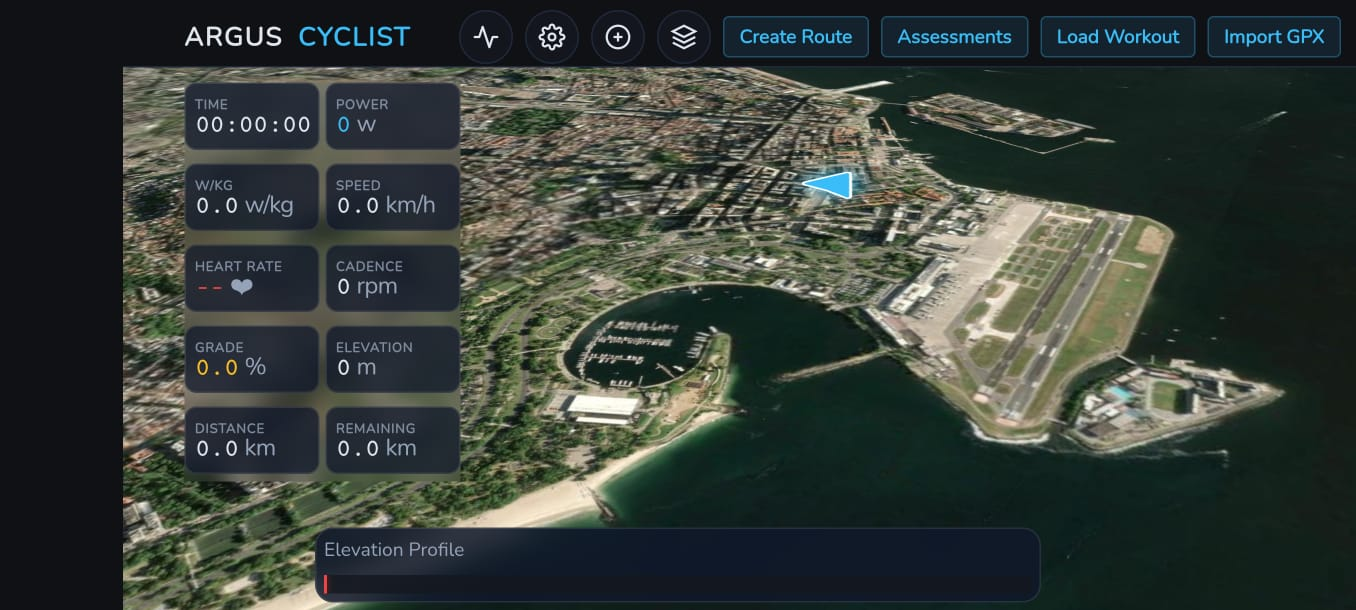
\includegraphics[width=0.85\textwidth]{figuras/screenshot-10-mobile}
    \caption{Aplicativo Android: HUD de simulação em modo \textit{landscape}}
    \label{fig:screenshot-mobile}
    \small Fonte: autoria própria.
\end{figure}

A física móvel é uma reimplementação, não um porte do motor Go. O código
JavaScript usa Newton--Raphson, coeficiente de rolamento 0,004 e eficiência de
transmissão 0,97; o desktop usa bisseção, coeficiente 0,005 e eficiência 0,96.
O parser GPX móvel usa distância horizontal e uma janela de suavização menor.
Essas diferenças são visíveis em uma comparação lado a lado e impedem afirmar
que as duas plataformas executam o mesmo modelo. O que é compartilhado é a
interface, a intenção de simulação e o formato de percurso; o núcleo de cálculo
é distinto.

O modo móvel também não oferece o rolo virtual, os testes de aptidão, a
exportação FIT, o histórico, o Strava ou o Intervals.icu. O código exibe um
aviso explícito de que a versão móvel suporta métricas ao vivo e que o
salvamento FIT está disponível no desktop. A arquitetura móvel é, portanto, um
modo complementar de sessão, não uma paridade funcional. A palavra
``multiplataforma'' no título se sustenta pela execução em Windows, Linux e
Android; ela não promete que todos os recursos existam em todas as plataformas.

O projeto iOS/iPadOS existe na estrutura Capacitor, mas não foi compilado,
assinado ou executado neste trabalho. O layout para tablet Android foi
projetado com \textit{breakpoints}, mas não foi testado em dispositivo físico.
macOS é compilável pelo Wails, mas não foi validado. A
Tabela~\ref{tab:plataformas-arquitetura} separa o que é decisão de projeto do
que é evidência de execução.

\begin{table}[htbp]
    \centering
    \caption{Status arquitetural das plataformas}
    \label{tab:plataformas-arquitetura}
    \small
    \begin{tabular}{@{}>{\raggedright\arraybackslash}p{2.8cm}
        >{\raggedright\arraybackslash}p{5.2cm}
        >{\raggedright\arraybackslash}p{4.0cm}@{}}
        \toprule
        \textbf{Plataforma} & \textbf{O que existe} & \textbf{Status} \\
        \midrule
        Windows e Linux & Wails, Go, BLE, SQLite, FIT e integrações &
        Validado \\
        Android & Capacitor, BLE nativo, GPX, física JS, sessão ao vivo &
        Validado como modo ao vivo; sem FIT/histórico \\
        iOS/iPadOS & Estrutura Capacitor preparada & Não compilado nem
        validado \\
        Tablet Android & Layout responsivo projetado & Não testado em
        dispositivo \\
        macOS & Projeto Wails e código portável & Não validado \\
        \bottomrule
    \end{tabular}
    \vspace{0.2cm}
    \par\small Fonte: autoria própria.
\end{table}

\section{Desktop, WebView e navegador}
\label{sec:desktop-browser}

O \argus{} desktop não é uma aplicação web aberta no navegador. O Wails embute
os arquivos do \textit{frontend} em um WebView do sistema e expõe métodos Go
por uma ponte. Essa escolha traz três vantagens: acesso nativo a BLE e ao
sistema de arquivos, persistência SQLite sem um servidor e distribuição em um
executável. O custo é a dependência do WebView de cada sistema e a necessidade
de manter uma ponte entre duas linguagens.

Uma versão somente para navegador teria outras restrições. A Web Bluetooth API
está disponível em navegadores baseados em Chromium, exige contexto seguro e
um gesto do usuário, e não oferece a mesma liberdade de acesso em segundo
plano. O armazenamento local do navegador não é equivalente a um arquivo
SQLite gerenciado pelo aplicativo, e o acesso a arquivos GPX/FIT depende de
seleção manual. Por outro lado, uma versão web teria instalação zero e
atualização centralizada. O \argus{} não escolheu esse caminho porque o controle
de hardware e o arquivo local são centrais para a proposta. A
Tabela~\ref{tab:desktop-browser} resume a comparação.

A escolha por Wails também poderia ser comparada a Electron e Tauri. Electron
embutiria um runtime Node/Chromium adicional; Tauri usaria um núcleo Rust e um
WebView. O \argus{} já tinha o núcleo em Go e uma biblioteca BLE nessa
linguagem, de modo que Wails reduziu a distância entre o núcleo e a interface.
Não foi realizado um comparativo de consumo de memória ou de tamanho de
binário; a decisão é de adequação ao código existente, não de \textit{benchmark}.

\begin{table}[H]
    \centering
    \caption{Comparação entre o aplicativo desktop e uma versão somente web}
    \label{tab:desktop-browser}
    \small
    \begin{tabular}{@{}>{\raggedright\arraybackslash}p{3.0cm}
        >{\raggedright\arraybackslash}p{5.0cm}
        >{\raggedright\arraybackslash}p{5.0cm}@{}}
        \toprule
        \textbf{Critério} & \textbf{Desktop (Wails)} & \textbf{Navegador} \\
        \midrule
        BLE & TinyGo, acesso nativo & Web Bluetooth, com restrições de
        navegador e de permissão \\
        Arquivos e SQLite & Acesso direto ao sistema de arquivos & OPFS ou
        IndexedDB; importação manual de arquivos \\
        Segundo plano & Processo nativo & Limitado pelo navegador \\
        Distribuição & Executável por plataforma & URL, sem instalação \\
        Atualização & Nova versão do aplicativo & Imediata no servidor \\
        Offline & Sim, exceto tiles e integrações & Depende de cache e de
        service worker \\
        \bottomrule
    \end{tabular}
    \vspace{0.2cm}
    \par\small Fonte: autoria própria.
\end{table}

\section{Segurança, privacidade e \textit{local-first}}
\label{sec:seguranca}

O modelo de segurança é o de uma aplicação pessoal local. Não há conta remota
obrigatória, servidor de autenticação ou banco central. Os dados de treino ficam
no SQLite do dispositivo; as integrações com Strava e Intervals.icu são opcionais
e usam OAuth ou chave de API fornecida pelo usuário. O assistente de IA acessa
um Ollama local em \code{127.0.0.1:11434}. Os \textit{tiles} do mapa e as APIs
externas são as principais saídas de rede.

Essa arquitetura reduz a exposição, mas não elimina riscos. Os tokens e a chave
de API ficam em texto simples no SQLite; não há criptografia em repouso nem
\textit{keyring} do sistema. As permissões do arquivo dependem do sistema
operacional e do diretório de instalação. Os perfis locais não são contas
protegidas por senha; a troca de perfil é uma conveniência, não um controle de
acesso. Em um computador compartilhado, outra pessoa com acesso ao mesmo
usuário do sistema pode ler os dados. O mapa depende de um serviço remoto de
tiles; a expressão ``local-first'' se aplica ao dado e ao processamento, não à
visualização completa.

O trabalho não implementa \textit{backup} automático, sincronização entre
dispositivos, resolução de conflitos ou criptografia ponta a ponta. Essas
funções seriam necessárias para um uso multiusuário ou corporativo; para o
escopo atual, a prioridade foi manter o dado sob controle do usuário e evitar
dependência de nuvem. A Seção~\ref{sec:limitacoes-resultados} retoma essas
ausências como limitações.

\section{Decisões e compensações}
\label{sec:tradeoffs}

A Tabela~\ref{tab:adr} registra as decisões arquiteturais mais relevantes no
formato de decisão, justificativa e consequência. Ela não substitui os
registros de \textit{commit}, mas dá ao leitor uma visão compacta do raciocínio.

A decisão mais custosa é a duplicação da física e do parser GPX no Android.
Ela foi aceita porque o Capacitor não executa Go e porque portar o núcleo Go
para WebAssembly exigiria uma cadeia de compilação e uma ponte adicionais que
não estavam no escopo. O resultado é uma plataforma móvel funcional para sessão
ao vivo, mas não equivalente ao desktop. A alternativa ``um único núcleo em
todas as plataformas'' continua sendo o caminho mais coerente para trabalhos
futuros, seja por WebAssembly, seja por um \textit{backend} embarcado.

A ausência de um servidor próprio também é uma escolha, não uma falha. Um
servidor permitiria sincronização, contas e comparação entre atletas, mas
introduziria custo operacional, autenticação, LGPD e disponibilidade. Para um
artefato de TCC com foco em percurso e dado local, o monólito modular é
suficiente e mais fácil de auditar. O limite aparece quando o uso cresce: o
SQLite por dispositivo não resolve colaboração, e o upload manual não substitui
uma fila de sincronização.

\begin{table}[H]
    \centering
    \caption{Decisões arquiteturais e consequências}
    \label{tab:adr}
    \footnotesize
    \renewcommand{\arraystretch}{1.12}
    \begin{tabular}{@{}>{\raggedright\arraybackslash}p{1.2cm}
        >{\raggedright\arraybackslash}p{4.0cm}
        >{\raggedright\arraybackslash}p{4.2cm}
        >{\raggedright\arraybackslash}p{4.2cm}@{}}
        \toprule
        \textbf{ID} & \textbf{Decisão} & \textbf{Motivo} & \textbf{Consequência} \\
        \midrule
        ADR-01 & Go + Wails no desktop & Núcleo Go, BLE e binário único &
        WebView dependente do sistema; ponte JS/Go \\
        ADR-02 & SQLite local por perfil & Controle do dado e isolamento &
        Sem sincronização; migrações simples; tokens em texto \\
        ADR-03 & Porta \code{TrainerService} & Trocar BLE, virtual e mock &
        Comportamento do hardware não é abstraído \\
        ADR-04 & Telemetria por eventos & Não bloquear a interface &
        Taxa variável; sem reamostragem \\
        ADR-05 & FE-C sobre BLE & Compatibilidade com rolos que o
        expõem & Não é ANT+ nativo; configuração fixa \\
        ADR-06 & Android via Capacitor & Reuso da interface & Física e GPX
        duplicados; sem FIT/histórico \\
        ADR-07 & IA via Ollama & Privacidade e operação local & Modelo pequeno;
        validação apenas sintática \\
        ADR-08 & Monólito modular & Escopo de TCC e uma equipe & Acoplamento em
        \code{app.go}; sem escala horizontal \\
        \bottomrule
    \end{tabular}
    \vspace{0.2cm}
    \par\small Fonte: autoria própria.
\end{table}

\section{Síntese do capítulo}
\label{sec:sintese-arquitetura}

A arquitetura do \argus{} é uma arquitetura de compromissos explícitos. O
desktop concentra o núcleo Go, a persistência, a exportação e as integrações; o
Android oferece um modo de sessão ao vivo com física e GPX próprios; a interface
é compartilhada, mas o núcleo não é. A separação em portas e adaptadores
permitiu trocar rolo, repositório e transporte, mas não eliminou a
dependência de SQLite na fachada nem a concentração de orquestração em
\code{app.go}. O capítulo seguinte mostra como essas decisões aparecem no
código e quais são as consequências práticas para a sessão, a exportação e a
análise.
